\documentclass[referee]{gji}
\usepackage{timet,color}
\usepackage{graphicx}
\usepackage{amsmath}
\usepackage{amssymb}
\usepackage{booktabs}
\usepackage{longtable}
\usepackage{url}
\usepackage[switch]{lineno}
\makeatletter
\let\bibhang\relax
\makeatother
\usepackage{gji_extra}
\usepackage[hidelinks]{hyperref}
\newcommand{\figalt}[1]{\par\smallskip\noindent\textit{Alt text:} #1}

\title[Probabilistic surface-wave inversion]
  {Probabilistic Surface-Wave Dispersion Inversion with a Depth-Controlled Conditional Rectified Flow}

\author[X. Liu et al.]
  {Xin Liu$^1$, Ziye Yu$^1$\thanks{Corresponding author: yuziye@cea-igp.ac.cn}
  and Yuqi Cai$^1$\\
  $^1$Institute of Geophysics, China Earthquake Administration, Beijing 100081, China
  }

\date{}
\pagerange{\pageref{firstpage}--\pageref{lastpage}}
\volume{000}
\pubyear{2026}

\let\leqslant=\leq

\begin{document}
\label{firstpage}
\maketitle
\linenumbers
\pagestyle{plain}

\begin{summary}
Surface-wave dispersion inversion is non-unique, but deterministic neural inversions usually return only a point estimate. We develop an amortised probabilistic inversion in which a depth-controlled conditional rectified flow samples ensembles of 1-D $V_P$, $V_S$ and density profiles conditioned on incomplete Rayleigh/Love phase-velocity curves. The learned distribution is a posterior surrogate for the specified synthetic prior, forward solver, observation mask, mask-only noise model and depth-control basis; it is not a universal field-data posterior.

Matched DI-Strong and DI-Weak samplers are trained from scratch with identical budgets so that only the structural prior generator differs. In the $N=1024$ in-prior diagnostic, DI-Strong reaches posterior-median $V_S$ MAE of 0.086 km s$^{-1}$ and mean pointwise 16--84 per cent interval coverage of 0.638. The prior-support audit shows the expected trade-off: DI-Weak reduces boundary and out-of-prior $V_S$ MAE to 0.171 and 0.499 km s$^{-1}$, compared with 0.372 and 0.782 km s$^{-1}$ for DI-Strong, while losing in-prior accuracy. Split-sample posterior-temperature scaling improves held-out mean coverage but is only a calibration diagnostic, not an observational likelihood. A Rayleigh-only Bayan Obo subarray MASW example \citep{Yang2025BayanOboDataset} demonstrates how local posterior ensembles can be assembled into pseudo-3-D workflow summaries; because the field example has no Love waves, no field likelihood and no independent calibration set, it is not interpreted as calibrated geological uncertainty.
\end{summary}

\begin{keywords}
Inverse theory -- Probability distributions -- Neural networks -- Surface waves and free oscillations -- Seismic velocities -- Computational seismology.
\end{keywords}

\section{Introduction}

Geophysical inverse problems are rarely one-to-one. Surface-wave dispersion curves constrain weighted averages of elastic structure over period-dependent depth ranges, and many velocity models can explain similar observations. Classical inverse-problem theory therefore treats the answer as a posterior probability distribution rather than as a single preferred model \citep{MosegaardTarantola1995,Tarantola2005}. In surface-wave applications, stochastic and transdimensional methods have made this non-uniqueness explicit by mapping trade-offs among layer velocities, discontinuity depths, smoothing assumptions and data errors \citep{Sambridge1999,ShapiroRitzwoller2002,BodinEtAl2012,GaoLekic2018}. A useful inversion method should therefore report not only a central model but also uncertainty summaries that can be checked against known synthetic truth or independent constraints.

The computational cost of repeated forward modelling motivates learned inversion. A deep neural network (DNN) can be trained on synthetic pairs of Earth models and dispersion curves, and then used as an amortised inverse map. Ordinary deterministic DNN inversions, however, tend to return point estimates and can hide the non-uniqueness that motivates Bayesian inversion in the first place. Earlier probabilistic neural approaches estimated crustal thickness or velocity-model uncertainty from surface waves \citep{DevileeEtAl1999,MeierEtAl2007}, and recent mixture-density and deterministic networks have extended the idea to field-scale dispersion inversion and near-surface applications \citep{EarpEtAl2020,KeilWassermann2023,ChenEtAl2022}. These methods are naturally viewed as simulation-based inference: a prior generator and a forward simulator define a prior-predictive distribution, and the network learns a conditional posterior surrogate for that distribution \citep{CranmerEtAl2020}.

Conditional rectified flow offers a direct way to represent this posterior surrogate as samples rather than as a single regressed profile. After training, different Gaussian initial states are transported to different elastic structures conditioned on the same dispersion curve. The resulting ensemble can be summarised by posterior medians, pointwise 16--84 per cent intervals, posterior standard deviations and posterior density views. Those summaries are useful only if their calibration is tested, because a visually plausible ensemble can still be too narrow, too broad or biased by the training distribution.

The novelty of the present workflow is the combination of four elements that are usually treated separately. Compared with deterministic DNN inversion, it returns posterior samples rather than only a regressed model. Compared with mixture-density networks, it uses a continuous depth-control transport map that can be sampled repeatedly at full-grid resolution. Compared with generic invertible-network or flow demonstrations, it reports surface-wave-specific posterior-predictive residuals, depth-binned coverage, reliability and rank diagnostics. Compared with conventional Bayesian inversion, it amortises sampling after training but keeps the prior-predictive assumptions explicit and auditable.

This paper develops a probabilistic direct-inversion workflow based on a depth-controlled conditional rectified flow. The main scientific object is the learned posterior surrogate $q_\theta({\bf m}|{\bf d})$, where ${\bf m}$ is a 1-D elastic structure and ${\bf d}$ is a masked Rayleigh/Love dispersion vector. We ask four questions. First, what posterior object does a DNN learn when trained on synthetic prior-predictive examples? Second, can a depth-controlled conditional flow produce regular posterior samples while preserving full-grid evaluation? Third, can posterior uncertainty be assessed using empirical coverage and calibration diagnostics? Fourth, how sensitive is the learned posterior to prior support?

The central result is that a depth-controlled conditional rectified flow can provide fast posterior ensembles for surface-wave dispersion, but the ensemble must be interpreted under its prior-predictive construction. The prior is not only a philosophical assumption written in an equation. In a DNN inversion workflow it is encoded by the synthetic model generator, velocity and density bounds, depth clipping, layer or control-point parameterisation, wave-type availability, observation masks and noise augmentation. The complete workflow is summarized in Fig.~\ref{fig:workflow}. We therefore include a matched prior-support stress test comparing strong- and weak-prior samplers trained with the same budget. The purpose is not to argue that weak priors are always better. It is to show that DNN posterior uncertainty can be sampled, tested, calibrated and audited within a defined synthetic inversion problem.

\section{Posterior target and prior-predictive construction}

\subsection{Bayesian object learned by the DNN}

Let ${\bf m}$ denote the 1-D model state and ${\bf d}$ the dispersion observation. The formal Bayesian target is
\begin{equation}
p({\bf m}|{\bf d}) \propto p({\bf d}|{\bf m})p({\bf m}),
\label{eq:bayes}
\end{equation}
but in the learned workflow neither term is evaluated analytically during inference. Instead, training pairs are generated by
\begin{equation}
\begin{split}
{\bf m}&\sim p_{\rm syn}({\bf m}),\qquad
{\bf q}\sim p_{\rm mask}({\bf q}),\\
{\bf d}&=\mathcal{E}_{\bf q}\left[\mathcal{F}({\bf m})+\boldsymbol{\epsilon}\right],
\qquad
\boldsymbol{\epsilon}\sim p_\epsilon .
\end{split}
\label{eq:priorpredictive}
\end{equation}
Here $p_{\rm syn}$ is the synthetic structural prior, $\mathcal{F}$ is the Rayleigh/Love forward solver, ${\bf q}$ is the observation mask, $\mathcal{E}_{\bf q}$ encodes the masked data vector and $p_\epsilon$ is the assumed synthetic observation-error distribution. In the present benchmark no additive phase-velocity noise is applied, so $p_\epsilon$ is a point mass at zero and the stochastic observation process is the masking operation. These choices define a training joint distribution $p_{\rm train}({\bf m},{\bf d})$ and a conditional distribution $p_{\rm train}({\bf m}|{\bf d})$. The DNN learns a posterior surrogate $q_\theta({\bf m}|{\bf d})$ for this conditional law.

Throughout this paper, posterior probability means probability under the stated prior-predictive construction. It is not a calibrated posterior for arbitrary field dispersion measurements unless the field data are represented by a suitable observational error model and the posterior is independently calibrated. This distinction is the reason for treating prior support as a reliability audit rather than as a data-generation detail.

\begin{figure*}
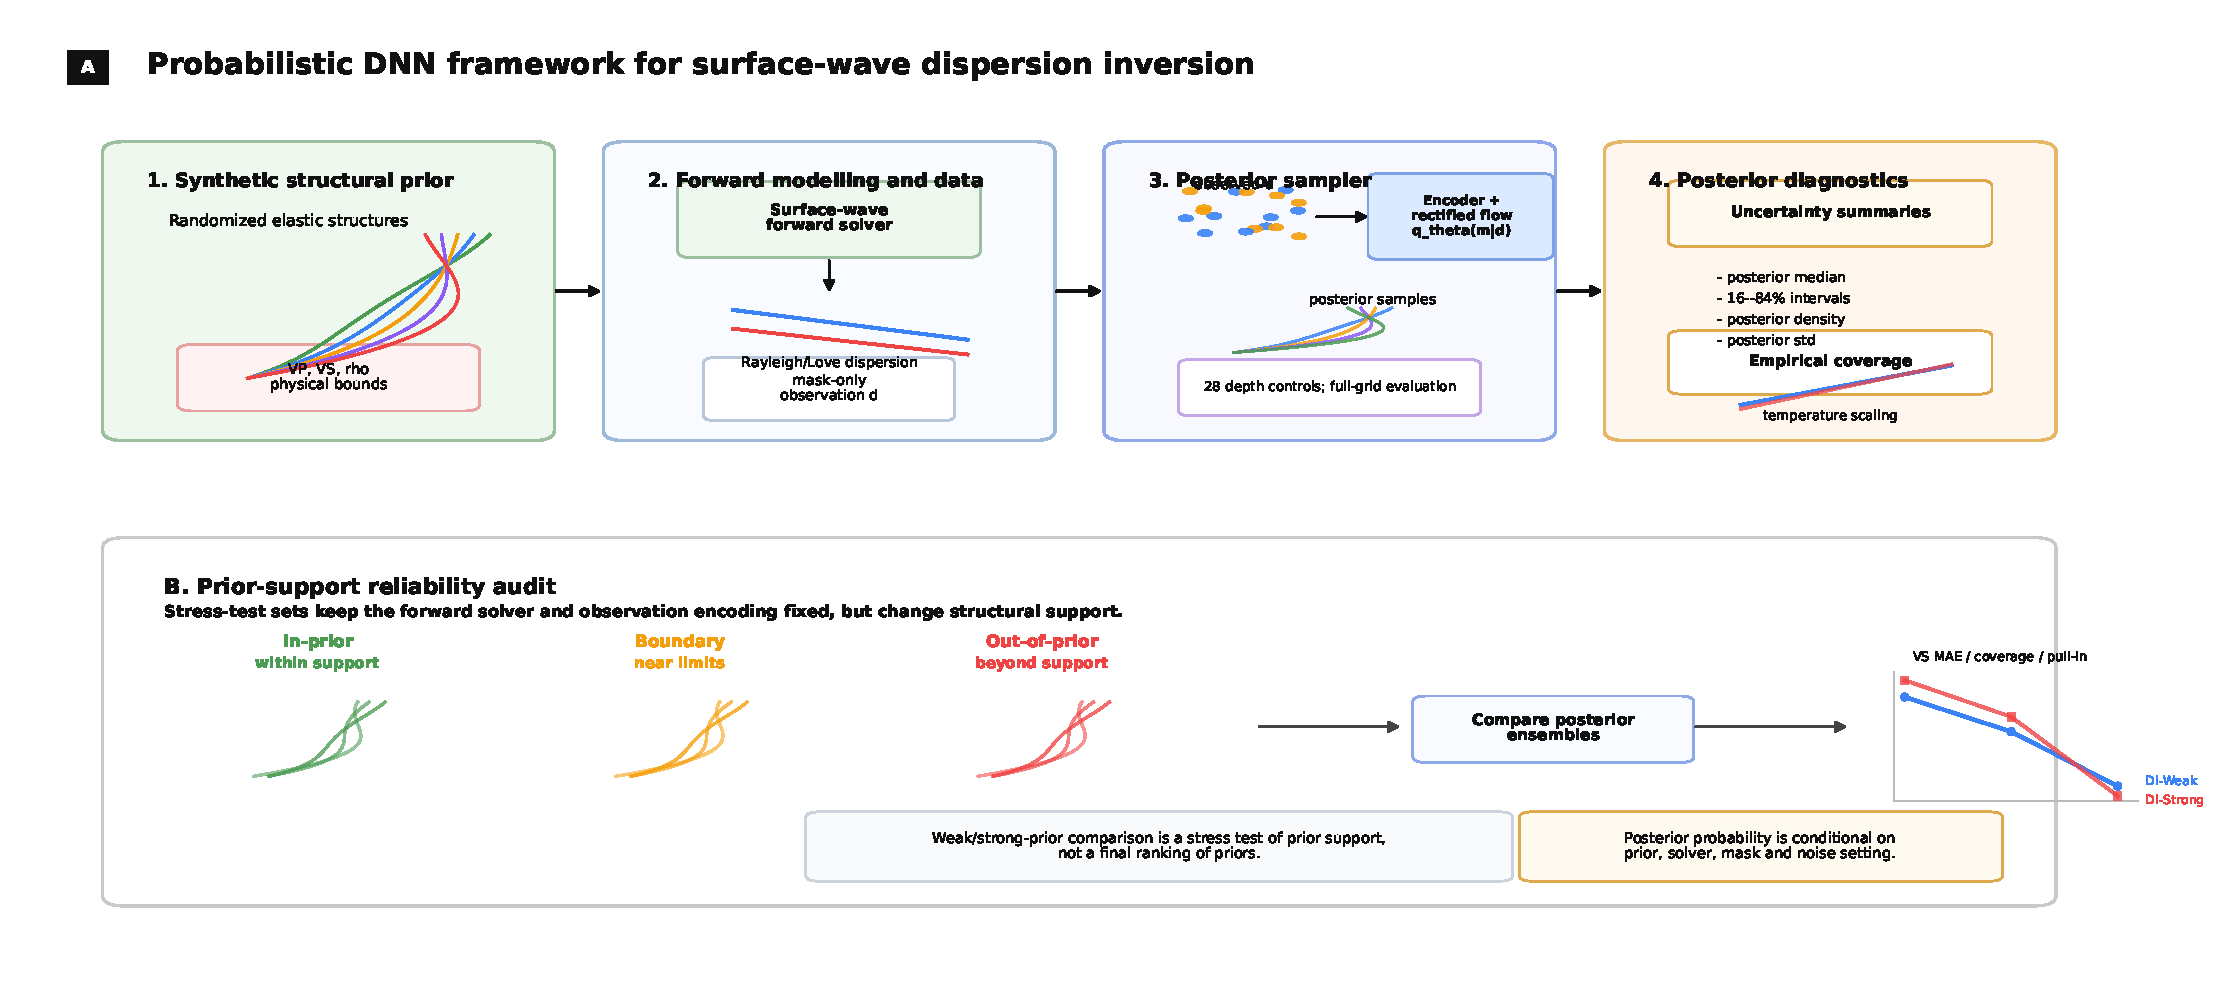
\includegraphics[width=\textwidth]{figures/fig01_dnn_posterior_workflow.pdf}
\caption{Schematic overview of probabilistic direct inversion using a depth-controlled conditional rectified flow. (A) A synthetic structural prior and a surface-wave forward solver define the prior-predictive training distribution for posterior inversion. A conditional rectified-flow network learns the direct posterior sampler $q_\theta({\bf m}|{\bf d})$, and posterior diagnostics summarise samples, medians, pointwise credible intervals, empirical coverage, calibration and prior-boundary pull-in. (B) The diagnostic test sets contain in-prior, boundary and out-of-prior structures while keeping the forward solver and observation encoding fixed. (C) Matched DI-Strong and DI-Weak samplers are compared only as a prior-support audit, using $V_S$ error, dispersion residual, coverage and pull-in. (D) Example profiles illustrate posterior medians and 16--84 per cent intervals. (E) Posterior probability is interpreted under the chosen prior, simulator, mask and noise model; calibration is required before field-data probability claims.}
\figalt{A five-panel workflow diagram linking synthetic structural priors, surface-wave forward modelling, conditional-flow posterior sampling, prior-support stress tests, example posterior profiles and uncertainty diagnostics.}
\label{fig:workflow}
\end{figure*}

\subsection{Diagnostic weak-prior generator}

The weak-prior diagnostic sampler uses a broad structural prior. This generator uses broad depth-dependent bounds rather than explicit tectonic classes, Moho templates or prescribed low-velocity-zone forms. It expands admissible ranges for $V_P$, $V_S$, density, sediment thickness, Moho depth, upper-mantle velocity, and low-velocity-zone depth and amplitude while retaining physical constraints such as $V_P>V_S$, positive $V_S$ and reasonable density. Random control points and weakly correlated perturbations allow a wider family of smooth profiles.

The weak prior is not prior-free. It still imposes velocity bounds, smoothness preferences, physical consistency rules and a depth basis. Its purpose is to make the learned posterior less dependent on narrow tectonic templates and less likely to exclude plausible structures before inversion. Because the same dispersion observation is compatible with a broader set of models, a weak-prior posterior should also be broader and harder to learn from finite training data. This is the intended trade-off tested below.

\subsection{Strong structural prior as a narrow-prior control}

The strong-prior control is generated from a synthetic 1-D tectonic model prior. Each sample contains depth, $V_P$, $V_S$ and density on a regular 0.5 km grid. Five broad tectonic classes are sampled: oceanic, shield, platform, orogen and rift. Each class defines ranges for crustal thickness, sediment thickness, upper- and lower-crustal $V_S$, upper-mantle $V_S$, and the probability, depth and amplitude of an upper-mantle low-velocity zone. $V_P$ is generated from layer-dependent $V_P/V_S$ ratios, and density is computed from empirical crustal relations \citep{Brocher2005}. This prior is geologically structured and useful for stabilising inversion, but it is deliberately bounded. We use it to quantify what is gained and lost when the direct posterior sampler is trained on a narrow prior.

Appendix Table~\ref{tab:priorparameters} lists the main parameter ranges used by the two generators. These values are not fitted to the field data in this manuscript; they define the synthetic prior-predictive problem used to train and test $q_\theta({\bf m}|{\bf d})$.

For both priors, the full model vector is
\begin{equation}
{\bf m}(z)=\{V_P(z),V_S(z),\rho(z)\},
\end{equation}
sampled at 256 depth nodes, giving a maximum represented depth of 127.5 km. The depth coordinate is fixed. Surface-wave phase velocities are computed for periods from 2 to 60 s using a Python implementation of surface-wave dispersion routines based on Computer Programs in Seismology \citep{Herrmann2013,LuuDisba}. The observation vector contains normalised period, Rayleigh velocity, Love velocity and separate masks for the two wave types. Missing velocities are set to zero after normalisation and are identified by the masks.

\subsection{Depth-control representation}

Although the posterior is evaluated on the full 256-node grid, the DNN samples values at 28 depth controls and then linearly interpolates to the full grid. Weak-prior examples and the 28-control basis are shown in Fig.~\ref{fig:controlpoints}. The controls are dense near the surface and sparse at depth: 0--5 km every 0.5 km, 5--10 km every 1 km, 10--50 km every 5 km and 50--127.5 km every 20 km. Let ${\bf m}_{\rm cp}$ be the vector of $V_P$, $V_S$ and density at these control depths. The full profile is
\begin{equation}
{\bf m}(z_i)=\mathcal{I}\left[{\bf m}_{\rm cp}\right](z_i),
\end{equation}
where $\mathcal{I}$ is a fixed differentiable interpolation operator. This basis is part of the prior-predictive definition because it restricts the stochastic degrees of freedom available to the posterior sampler.

\begin{figure}
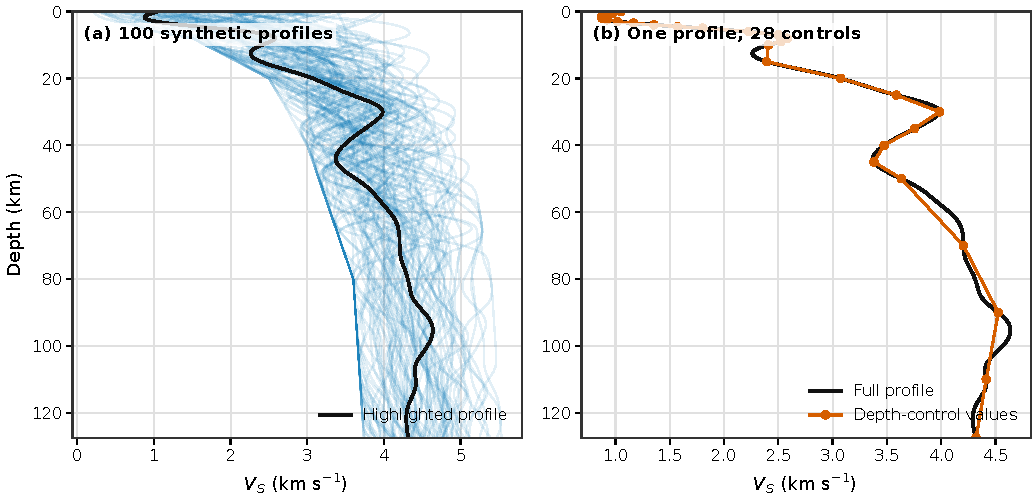
\includegraphics[width=\columnwidth]{figures/fig02_control_points.pdf}
\caption{Weak-prior examples and the depth-control basis used by the DNN posterior sampler. (a) One hundred synthetic $V_S$ profiles drawn from the weak structural prior. (b) The network samples $V_P$, $V_S$ and density at 28 control depths; profiles are interpolated to the full 256-node grid for loss evaluation, posterior summaries and metrics.}
\figalt{Line plots showing broad weak-prior shear-velocity profiles and the corresponding nonuniform depth-control points that are dense near the surface and sparse at depth.}
\label{fig:controlpoints}
\end{figure}

\section{DNN posterior sampler}

\subsection{Conditioning encoder}

The conditional input has five period-indexed channels: normalised period, normalised Rayleigh phase velocity, normalised Love phase velocity, Rayleigh mask and Love mask. A one-dimensional convolutional encoder with residual blocks maps this input to a 256-dimensional conditioning vector. The encoder sees both measured velocities and the pattern of missing observations, so the posterior sampler can represent cases with Rayleigh only, Love only, both wave types or incomplete period windows.

\subsection{Conditional rectified flow}

The depth-control target ${\bf m}_{\rm cp}$ is normalised by the training-set mean and standard deviation to form ${\bf z}_{\rm cp}$. During training, a Gaussian sample $\boldsymbol{\epsilon}\sim N(0,I)$ and a time $t\sim U(0,1)$ define the straight-line interpolation
\begin{equation}
{\bf x}_t=(1-t)\boldsymbol{\epsilon}+t{\bf z}_{\rm cp}.
\end{equation}
The velocity field $v_\theta({\bf x}_t,t,{\bf d})$ is trained to predict the displacement from noise to target:
\begin{equation}
\mathcal{L}_{\rm flow}=
\mathbb{E}\left[
\left\|v_\theta({\bf x}_t,t,{\bf d})-({\bf z}_{\rm cp}-\boldsymbol{\epsilon})\right\|_1
\right],
\label{eq:flowloss}
\end{equation}
implemented with a SmoothL1 loss. A one-step reconstruction term evaluates
\begin{equation}
\widehat{\bf z}_{\rm cp}={\bf x}_t+(1-t)v_\theta({\bf x}_t,t,{\bf d})
\end{equation}
and adds small first- and second-difference penalties after interpolation to the full depth grid. This encourages physically smooth posterior draws without post-processing the final samples.

After training, sampling starts from ${\bf x}_0\sim N(0,I)$ and integrates
\begin{equation}
\frac{d{\bf x}_t}{dt}=v_\theta({\bf x}_t,t,{\bf d})
\label{eq:ode}
\end{equation}
from $t=0$ to $t=1$. The endpoint is denormalised in control-point space and interpolated to the full grid. The push-forward distribution of the Gaussian source through this conditional ordinary differential equation is the learned posterior approximation $q_\theta({\bf m}|{\bf d})$. Rectified flow and related continuous-flow models provide an efficient way to learn such transport maps \citep{LiuGongLiu2022,LipmanEtAl2023}; invertible neural networks have been used similarly for ambiguous inverse problems \citep{ArdizzoneEtAl2019}.

\subsection{Training and posterior summaries}

DI-Strong and DI-Weak are trained from scratch with matched budgets: 100000 synthetic profiles, 2048 validation profiles, batch size 64, 24 scheduled epochs, the same encoder and conditional-flow architecture, the same optimizer and learning-rate schedule, the same loss weights, the same intermittent-band mask augmentation and the same random seed. The analysed checkpoint for each run is selected by validation total loss. The only intended difference is the structural prior generator. Unless otherwise stated, posterior summaries use 64 samples and 24 Euler steps. Point estimates are posterior medians computed independently at each depth and parameter, and uncertainty bands are pointwise marginal 16--84 per cent intervals from the sampled ensemble.

Empirical coverage is computed pointwise over model parameters and depths:
\begin{equation}
C_{16-84}=
\frac{1}{3ND}
\sum_{n=1}^{N}
\sum_{c=1}^{3}
\sum_{i=1}^{D}
{\bf 1}\left[
q_{0.16,nci}\le m^{\rm true}_{nci}\le q_{0.84,nci}
\right],
\label{eq:coverage}
\end{equation}
where $N$ is the number of evaluation examples, $D=256$ is the number of depth samples, $c$ indexes $V_P$, $V_S$ and density, and $q_{0.16}$ and $q_{0.84}$ are posterior-sample quantiles. This is marginal pointwise coverage, not the probability that an entire profile lies inside the plotted band.

We also use a simple split-sample posterior-temperature diagnostic. For each posterior sample ${\bf m}_s$ and pointwise posterior median $\widetilde{\bf m}$, the scaled sample is
\begin{equation}
{\bf m}^{(\tau)}_s=
\widetilde{\bf m}+\tau({\bf m}_s-\widetilde{\bf m}).
\label{eq:temperature}
\end{equation}
The scalar $\tau$ is fitted on a calibration subset to make mean pointwise 16--84 per cent coverage close to the nominal 0.68 target and is then evaluated on a held-out subset. This operation widens or narrows intervals without changing posterior medians. It is a diagnostic of posterior dispersion, not a replacement for a physical observational-error likelihood. The production result tables report the fitted temperature factors and held-out reliability curves for all methods and regimes.

\subsection{Prior-boundary diagnostic}

The prior-boundary diagnostic changes the test distribution while keeping the forward solver and observation format fixed. Three regimes are used. The in-prior set contains models drawn from the strong-prior generator. The boundary set places Moho depth, sediment thickness, upper-mantle $V_S$ and low-velocity-zone depth or amplitude close to the strong-prior limits. The out-of-prior set remains physically plausible but deliberately exceeds strong-prior support through thicker sediments, shifted Moho depths, stronger low-velocity zones, upper-mantle velocities outside default ranges or sharper gradients.

DI-Weak denotes the weak-prior conditional rectified-flow sampler and is the broad-prior configuration considered here. DI-Strong denotes the matched strong-prior sampler and is used as a narrow-prior control. Because DI-Strong and DI-Weak are trained with matched budgets, the numerical comparison isolates the structural-prior generator; it remains a prior-support audit rather than a universal prior ranking.

For each method and test regime we compute $V_P$, $V_S$ and density MAE, root-mean-square error, posterior interval coverage, forward-modelled dispersion residual and a prior-boundary pull-in statistic. The pull-in statistic estimates a pointwise 1--99 per cent envelope from the strong-prior training distribution. It then measures the fraction of target values outside that envelope whose posterior median is returned inside the envelope. Large pull-in indicates that the direct posterior map is drawing unfamiliar structures back into the strong-prior support.

\section{Results}

\subsection{Deep-learning posterior sampling performance}

The matched in-prior diagnostics show that the depth-controlled conditional rectified flow learns useful posterior surrogates under both structural priors (Table~\ref{tab:validation}; Fig.~\ref{fig:directexamples}). DI-Strong has lower in-prior median error, with $V_S$ MAE of 0.086 km s$^{-1}$ and mean 16--84 per cent coverage of 0.638. DI-Weak has broader structural support but higher in-prior error, with $V_S$ MAE of 0.134 km s$^{-1}$ and mean coverage of 0.577. The lower $V_S$ error relative to $V_P$ and density is expected because fundamental-mode surface-wave dispersion is most directly sensitive to shear velocity; $V_P$ and density are recovered mainly through prior correlations and physical constraints encoded in the synthetic generator.

\begin{table*}
\caption{Matched in-prior diagnostic statistics for DI-Strong and DI-Weak trained from scratch with identical budgets. Posterior summaries use 64 samples and 24 Euler steps. Coverage is mean pointwise 16--84 per cent interval coverage over $V_P$, $V_S$ and density; bootstrap confidence intervals are reported in the CSV/JSON result tables.}
\label{tab:validation}
\centering
\begin{tabular}{@{}lccccc@{}}
\toprule
Method & $N$ & $V_P$ MAE & $V_S$ MAE & Density MAE & Coverage \\
 & & (km s$^{-1}$) & (km s$^{-1}$) & (g cm$^{-3}$) & \\
\midrule
DI-Strong & 1024 & 0.235 & 0.086 & 0.079 & 0.638 \\
DI-Weak & 1024 & 0.333 & 0.134 & 0.150 & 0.577 \\
\bottomrule
\end{tabular}
\end{table*}

\begin{figure*}

\includegraphics[width=0.48\textwidth]{figures/fair_di_metric_summary.pdf}
\hfill
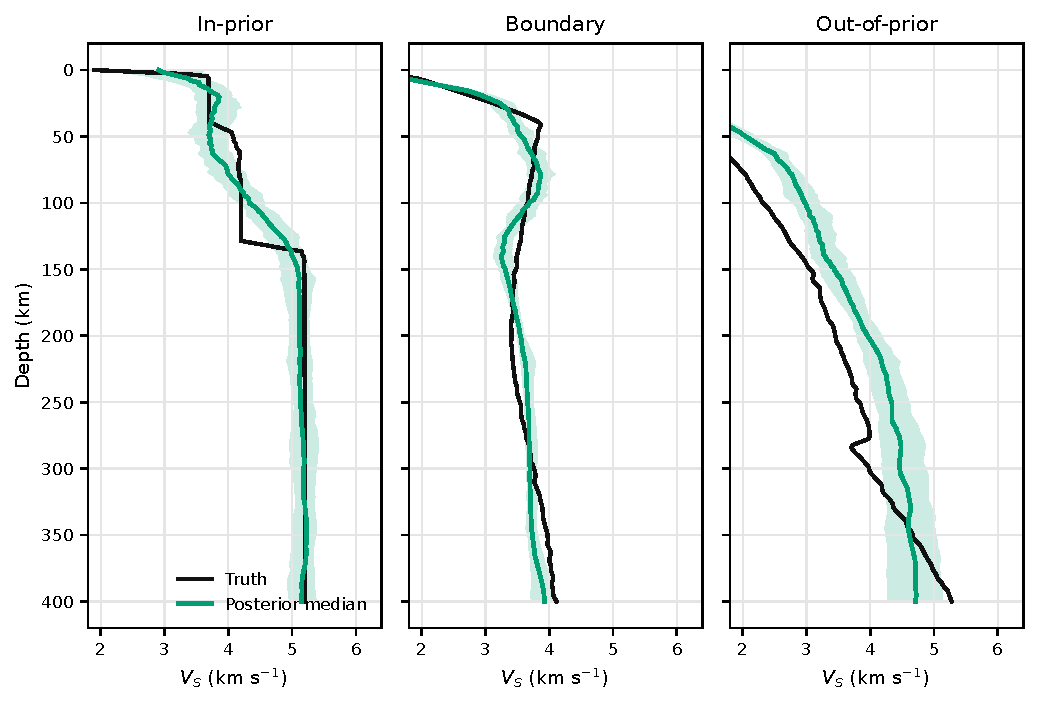
\includegraphics[width=0.48\textwidth]{figures/fair_di_example_profiles.pdf}
\caption{Matched production diagnostics for the conditional-flow posterior sampler. Left: metric summary for DI-Strong and DI-Weak on identical in-prior, boundary and out-of-prior test sets. Right: representative posterior profile examples with posterior medians and pointwise 16--84 per cent intervals.}
\figalt{Side-by-side plots of matched DI-Strong and DI-Weak performance metrics and representative velocity-density posterior profiles with median curves and 16--84 per cent intervals.}
\label{fig:directexamples}
\end{figure*}

\subsection{Empirical coverage and posterior-temperature calibration}

Raw posterior intervals are informative but not automatically calibrated (Fig.~\ref{fig:coverage}). On the in-prior held-out split, raw 68 per cent mean coverage is 0.631 for DI-Strong and 0.580 for DI-Weak. Scalar posterior-temperature scaling fitted on a separate calibration half gives held-out mean coverage of 0.681 and 0.685, with temperature factors of 1.114 and 1.316, respectively. Boundary and out-of-prior regimes require much larger corrections for DI-Strong ($\tau=3.160$ and 4.584), reflecting strong prior-support mismatch. DI-Weak needs smaller boundary correction ($\tau=1.687$) but still needs substantial out-of-prior widening ($\tau=3.335$). These results support the main claim that the DNN produces a sampleable posterior geometry, while also showing that empirical calibration is required before interpreting nominal intervals as probabilities.

Depth-binned coverage and rank diagnostics tell the same story with more spatial detail. For in-prior DI-Strong, raw depth-binned 68 per cent coverage ranges from 0.588 to 0.752 across channel-depth bins and becomes 0.641--0.795 after temperature scaling. DI-Weak has a wider raw in-prior range, 0.205--0.860, which becomes 0.258--0.941 after scaling; this indicates that one scalar temperature corrects the mean interval width but does not remove all depth- and parameter-dependent miscalibration. Rank/PIT histograms are also non-uniform before scaling: the two edge bins contain 0.201 of in-prior DI-Strong ranks and 0.281 of in-prior DI-Weak ranks, compared with 0.10 for a uniform diagnostic. The production result directory therefore includes both mean reliability curves and depth-binned/rank tables rather than relying on one aggregate coverage number.

\begin{figure}

\includegraphics[width=\columnwidth]{figures/fair_calibration_reliability.pdf}
\caption{Split-sample posterior-temperature diagnostic for the matched production samplers. Reliability curves compare empirical pointwise coverage against nominal credible interval levels on held-out examples. Temperature scaling changes posterior spread around the median but does not change the posterior median or replace an observational-error model.}
\figalt{Six reliability-curve panels for DI-Strong and DI-Weak across in-prior, boundary and out-of-prior regimes, comparing raw and temperature-scaled empirical coverage against nominal interval levels.}
\label{fig:coverage}
\end{figure}

\subsection{Missing period bands and posterior uncertainty}

The production samplers were trained with intermittent-band mask augmentation to better match incomplete dispersion picks. We evaluate the fair weak-prior checkpoint on 1024 synthetic examples using fixed and random period windows (Fig.~\ref{fig:missingband}). Reducing the mean valid fraction from 0.351 for the nominal 2--60 s mask to 0.235 for the 2--40 s window increases $V_S$ MAE from 0.164 to 0.192 km s$^{-1}$ and increases mean $V_S$ posterior spread from 0.179 to 0.206 km s$^{-1}$. The narrower 10--30 s window is more restrictive, with valid fraction 0.135, $V_S$ MAE 0.276 km s$^{-1}$ and mean $V_S$ spread 0.287 km s$^{-1}$. The random-window experiment has mean width 29.8 s, valid fraction 0.187, $V_S$ MAE 0.208 km s$^{-1}$ and mean spread 0.221 km s$^{-1}$.

The random-window examples provide an internal consistency check: valid fraction is negatively correlated with both posterior spread ($r=-0.577$) and $V_S$ MAE ($r=-0.440$). In other words, the posterior becomes broader and less accurate when less period support is available. Coverage remains below nominal but comparatively stable across the window choices, with mean 16--84 per cent coverage between 0.615 and 0.646. Missing-band augmentation therefore improves robustness to incomplete inputs, but calibration and an observational-error model remain necessary for probability claims.

\begin{figure*}

\includegraphics[width=0.48\textwidth]{figures/fair_missing_band_uncertainty.pdf}
\hfill
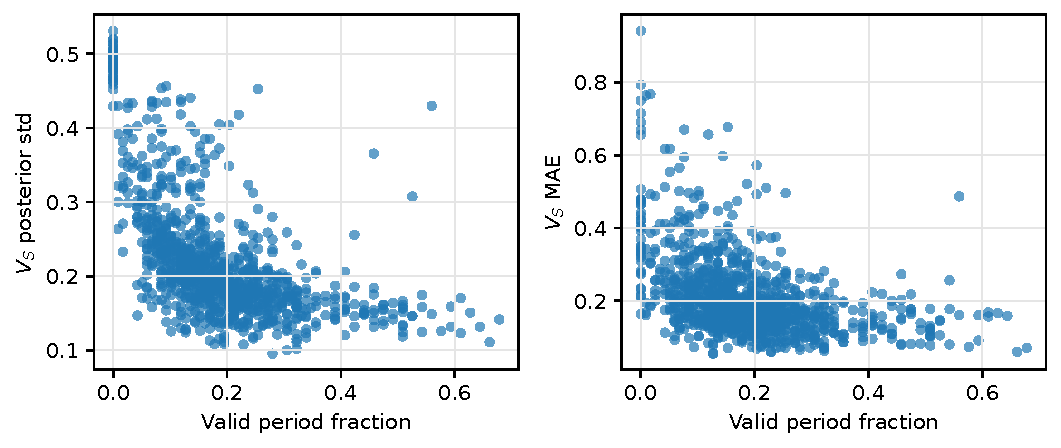
\includegraphics[width=0.48\textwidth]{figures/fair_missing_band_random_scatter.pdf}
\caption{Effect of missing period bands on weak-prior DNN posterior inversion. Left: fixed and random period-window diagnostics for posterior-median $V_S$ error, posterior spread and coverage. Right: random-window relationships between valid period fraction, posterior spread and error.}
\figalt{Bar charts and scatter plots showing that narrower or randomly incomplete period windows have lower valid-period fractions, larger shear-velocity errors and broader posterior spread.}
\label{fig:missingband}
\end{figure*}

\subsection{Evaluation-time phase-velocity noise}

The primary synthetic benchmark is mask-only, with no additive phase-velocity noise during training. We therefore treat additive noise as an evaluation-time sensitivity test rather than as a claim of noise-aware training (Fig.~\ref{fig:noise}). For in-prior DI-Weak, increasing Gaussian phase-velocity noise from 0 to 0.10 km s$^{-1}$ raises $V_S$ MAE from 0.133 to 0.299 km s$^{-1}$, raises mean posterior spread from 0.207 to 0.245, lowers mean raw coverage from 0.577 to 0.405 and increases the 68 per cent temperature factor from 1.336 to 2.053. DI-Strong shows the same trend, with in-prior $V_S$ MAE increasing from 0.086 to 0.199 km s$^{-1}$ and raw coverage falling from 0.638 to 0.394. This behaviour is expected: a sampler trained on a mask-only benchmark can recognise less consistent inputs through broader posterior summaries, but it has not learned a physical noise likelihood.

\begin{figure}

\includegraphics[width=\columnwidth]{figures/fair_noise_sensitivity.pdf}
\caption{Evaluation-time additive phase-velocity noise sensitivity. Gaussian noise is added only to observed Rayleigh/Love entries; masks and period channels are unchanged. The primary training condition remains the mask-only benchmark.}
\figalt{Line plots showing in-prior shear-velocity error, coverage, posterior standard deviation and temperature factor as additive phase-velocity noise increases from zero to 0.10 km per second.}
\label{fig:noise}
\end{figure}

\subsection{Prior-support reliability audit}

The prior-boundary experiment audits behaviour that is not visible from in-prior validation alone. It is a prior-support diagnostic rather than a final method ranking. DI-Weak reduces support-driven boundary collapse relative to DI-Strong (Table~\ref{tab:priorboundary}). Boundary $V_S$ MAE decreases from 0.372 km s$^{-1}$ for DI-Strong to 0.171 km s$^{-1}$ for DI-Weak, and out-of-prior $V_S$ MAE decreases from 0.782 to 0.499 km s$^{-1}$. Dispersion residuals decrease from 0.277 to 0.100 km s$^{-1}$ for boundary cases and from 0.335 to 0.262 km s$^{-1}$ for out-of-prior cases.

The pull-in statistic confirms that the improvement is a prior-support effect. For target values outside the strong-prior envelope, DI-Weak returns 0.101 of boundary predictions and 0.318 of out-of-prior predictions inside that envelope, compared with 0.725 and 0.815 for DI-Strong. The comparison demonstrates that the learned posterior depends on prior width: a broader prior can reduce boundary collapse, whereas the strong-prior control remains more accurate inside its own support.

\begin{table*}
\caption{Matched prior-support diagnostic for DI-Strong and DI-Weak trained from scratch with identical budgets. The table is a prior-support reliability audit, not a general ranking of priors. Pull-in is the fraction of target values outside the strong-prior envelope whose posterior medians return inside that envelope. Bootstrap confidence intervals are reported in the full result tables.}
\label{tab:priorboundary}
\centering
\begin{tabular}{@{}llccccc@{}}
\toprule
Method & Regime & $N$ & $V_S$ MAE & Disp. MAE & $V_S$ coverage & Pull-in \\
 & & & (km s$^{-1}$) & (km s$^{-1}$) & & \\
\midrule
DI-Strong & In-prior & 1024 & 0.086 & 0.030 & 0.660 & 0.803 \\
DI-Strong & Boundary & 1024 & 0.372 & 0.277 & 0.250 & 0.725 \\
DI-Strong & Out-of-prior & 1024 & 0.782 & 0.335 & 0.133 & 0.815 \\
DI-Weak & In-prior & 1024 & 0.134 & 0.049 & 0.786 & 0.706 \\
DI-Weak & Boundary & 1024 & 0.171 & 0.100 & 0.547 & 0.101 \\
DI-Weak & Out-of-prior & 1024 & 0.499 & 0.262 & 0.264 & 0.318 \\
\bottomrule
\end{tabular}
\end{table*}

\subsection{Baseline comparisons}

The deterministic DNN baselines use the same encoder/control representation and matched training budgets but return point estimates rather than posterior samples (Table~\ref{tab:baselines}; Fig.~\ref{fig:baselines}). They are competitive in median error: DET-Strong reaches in-prior $V_S$ MAE of 0.080 km s$^{-1}$ and DET-Weak reaches 0.127 km s$^{-1}$. Their limitation is not point-estimate accuracy, but the absence of posterior ensembles, empirical coverage and posterior calibration diagnostics. The learned-forward/optimization baseline (IND-FWD) was run as a computationally limited reference with $N=128$ per regime. It returns optimization ensembles and coverage estimates, but is slower and its dispersion residuals remain larger than the direct samplers in the reported setting.

\begin{table*}
\caption{Baseline diagnostic metrics. Deterministic DNN baselines are trained with matched budgets but do not produce posterior interval coverage. IND-FWD is a learned-forward/optimization reference run with $N=128$ per regime and is therefore interpreted as a computationally limited baseline rather than a final method ranking.}
\label{tab:baselines}
\centering
\begin{tabular}{@{}llcccc@{}}
\toprule
Method & Regime & $N$ & $V_S$ MAE & Disp. MAE & Coverage \\
 & & & (km s$^{-1}$) & (km s$^{-1}$) & \\
\midrule
DET-Strong & In-prior & 1024 & 0.080 & 0.045 & -- \\
DET-Strong & Boundary & 1024 & 0.399 & 0.307 & -- \\
DET-Strong & Out-of-prior & 1024 & 0.831 & 0.349 & -- \\
DET-Weak & In-prior & 1024 & 0.127 & 0.064 & -- \\
DET-Weak & Boundary & 1024 & 0.164 & 0.135 & -- \\
DET-Weak & Out-of-prior & 1024 & 0.429 & 0.240 & -- \\
IND-FWD & In-prior & 128 & 0.203 & 0.240 & 0.494 \\
IND-FWD & Boundary & 128 & 0.261 & 0.284 & 0.578 \\
IND-FWD & Out-of-prior & 128 & 0.369 & 0.384 & 0.478 \\
\bottomrule
\end{tabular}
\end{table*}

\begin{figure}

\includegraphics[width=\columnwidth]{figures/fair_baseline_metric_summary.pdf}
\caption{Baseline comparison for deterministic direct inversion and the learned-forward/optimization reference. Deterministic direct inversion gives point estimates only; conditional-flow DI adds posterior samples and calibration diagnostics.}
\figalt{Grouped bar charts comparing deterministic strong-prior, deterministic weak-prior and learned-forward optimization baselines by shear-velocity error and dispersion residual across three synthetic regimes.}
\label{fig:baselines}
\end{figure}

\subsection{Field demonstration on subarray MASW dispersion}

As a first field-data demonstration, we applied the matched DI-Weak sampler to subarray MASW Rayleigh-wave dispersion curves from the Bayan Obo data set \citep{Yang2025BayanOboDataset}. The data are used only to demonstrate the amortised posterior workflow on real incomplete dispersion picks. The MASW workflow provides one picked Rayleigh phase-velocity curve beneath each of 150 subarray centres. We converted each curve to the same period-indexed input used by the DNN, retained the 2--40 s period window and masked the Love-wave channel because Love dispersion was not available. The 40--60 s part of the automatic picks contains a nearly flat velocity segment close to the scanning limit, so it is excluded from this conservative demonstration rather than interpreted as a deep constraint.

The field run produces 64 posterior samples at every subarray centre. These local 1-D ensembles can be assembled into a pseudo-3-D velocity volume by mapping posterior medians and posterior standard deviations onto depth slices (Figs~\ref{fig:fieldmasw}--\ref{fig:fieldreference}). The mean number of retained periods is 39 per subarray. Mean posterior $V_S$ medians increase from 2.80 km s$^{-1}$ at 2 km to 3.81 km s$^{-1}$ at 20 km, then vary between 3.12 and 3.56 km s$^{-1}$ from 40 to 100 km. Mean posterior standard deviation is largest near the surface (0.458 km s$^{-1}$ at 2 km) and decreases below 60 km. Comparison against the available MASW-derived reference summary gives depth-dependent spatial correlations ranging from 0.139 at 2 km to 0.881 at 40 km and mean absolute $V_S$ differences from 0.027 to 0.361 km s$^{-1}$. Because no field-specific observational-error likelihood, Love-wave field measurements or independent calibration set is available, these numbers are interpreted as workflow diagnostics rather than calibrated geological uncertainty.

The depth interpretation is intentionally conservative. A 2--40 s Rayleigh-only input has limited independent sensitivity to deeper structure compared with a joint Rayleigh--Love, longer-period data set. Below the depth range directly supported by the available field dispersion picks, posterior medians and especially the decreasing posterior standard deviations are treated as prior-dominated summaries from the learned weak-prior workflow. We therefore do not interpret the deep slices as resolved deep mantle structure, and we do not describe the field standard deviations as field-calibrated observational uncertainty.

\begin{figure*}
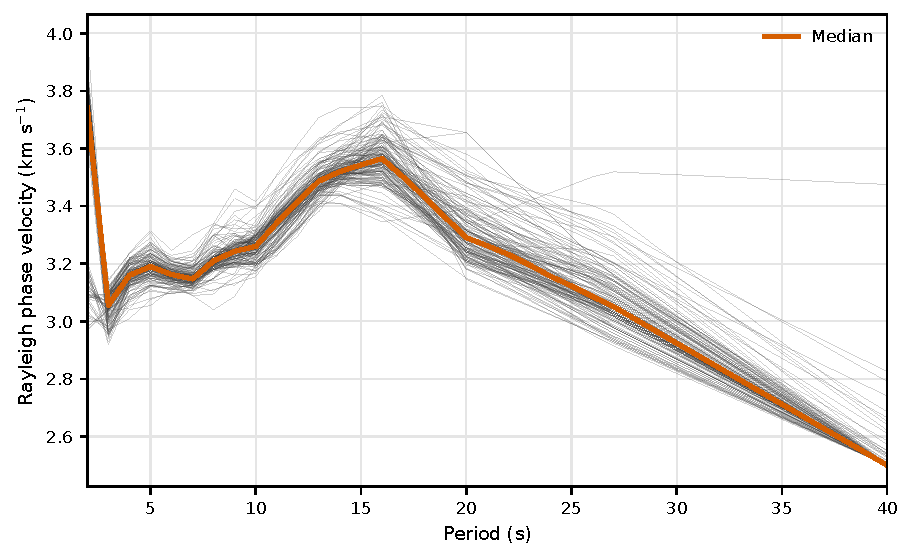
\includegraphics[width=0.48\textwidth]{figures/fair_field_dispersion_qc.pdf}
\hfill

\includegraphics[width=0.48\textwidth]{figures/fair_field_summary_vs_depth.pdf}
\caption{Field demonstration using Bayan Obo subarray MASW Rayleigh-wave dispersion curves \citep{Yang2025BayanOboDataset}. The fair weak-prior checkpoint is applied to 150 Rayleigh-only subarrays using 64 posterior samples and 24 Euler integration steps. Panels show dispersion quality control and depth summaries of posterior-median $V_S$, posterior standard deviation and comparison against the available MASW-derived reference summary.}
\figalt{Two field-summary panels showing quality control for Rayleigh-only dispersion picks and depth trends in posterior median shear velocity, posterior standard deviation and reference-model differences for 150 Bayan Obo subarrays.}
\label{fig:fieldmasw}
\end{figure*}

\begin{figure*}
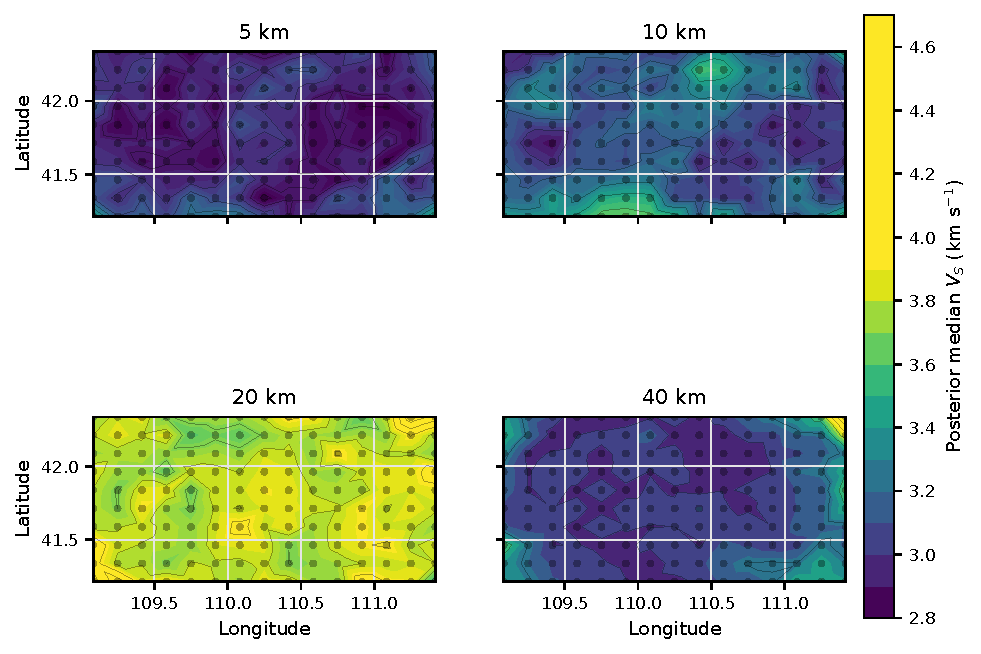
\includegraphics[width=0.48\textwidth]{figures/fair_field_vs_median_slices.pdf}
\hfill
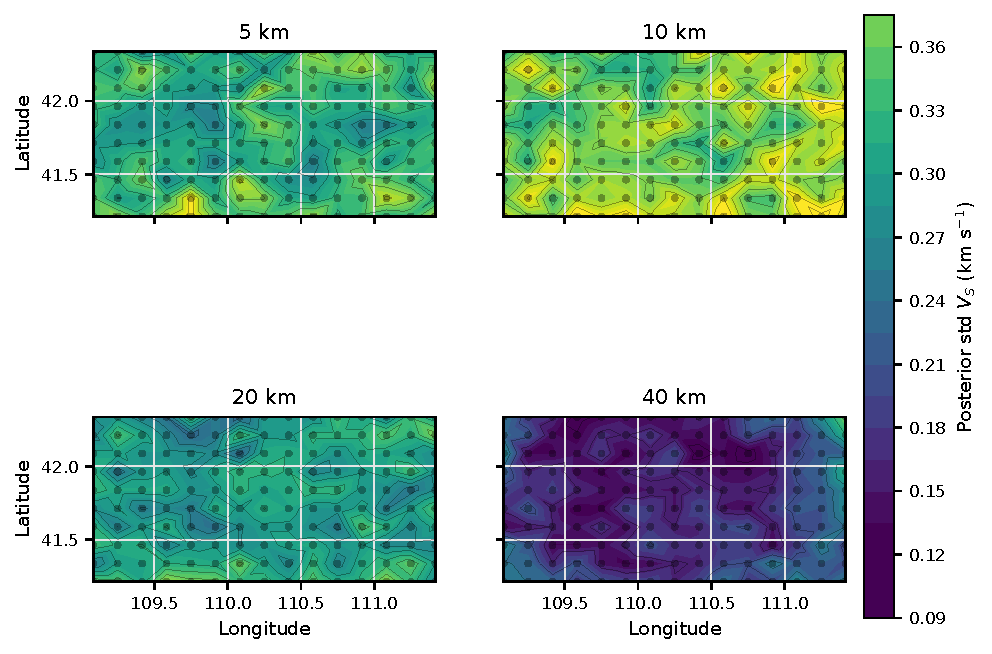
\includegraphics[width=0.48\textwidth]{figures/fair_field_vs_std_slices.pdf}
\caption{Pseudo-3-D field posterior summaries from the fair weak-prior checkpoint. Panels show posterior-median $V_S$ slices and posterior-standard-deviation slices. Because the benchmark has no field-specific observational-error likelihood and no Love-wave field measurements, posterior medians and posterior standard deviations are interpreted as workflow-level posterior summaries rather than field-calibrated uncertainty or a calibrated geological model.}
\figalt{Map slices of posterior median shear velocity and posterior shear-velocity standard deviation across the Bayan Obo subarray grid, displayed at multiple depths.}
\label{fig:fieldmaswslices}
\end{figure*}

\begin{figure}
\centering

\includegraphics[width=0.65\columnwidth]{figures/fair_field_reference_difference.pdf}
\caption{Depth-dependent comparison between the fair weak-prior field posterior medians and the available MASW-derived reference summary. This comparison is a field workflow diagnostic rather than an independent calibration of posterior probability.}
\figalt{Depth series comparing the DNN field posterior-median shear velocities with the available MASW-derived reference summary using correlation and difference metrics.}
\label{fig:fieldreference}
\end{figure}

\clearpage

\section{Discussion}

\subsection{Meaning of DNN posterior probability}

The posterior sampled by the DNN is a conditional distribution induced by a synthetic generator, a forward simulator, an observation mask, a noise model and a depth-control basis. This is a strength when those ingredients represent the intended inference problem: once trained, the sampler provides fast posterior draws, uncertainty summaries and posterior-predictive checks. It is also a limitation. Changing the structural generator, forward solver, masking process, observational error model or depth basis changes the posterior target being approximated.

This interpretation is important for field use. The DNN does not learn a universal inverse operator independent of assumptions; it learns a posterior surrogate for the training joint distribution. Posterior samples are therefore meaningful only together with the prior-predictive construction that produced them. Prior design, mask design, noise design and model parameterisation should be reported as part of the method, not hidden as data-generation details.

\subsection{Posterior uncertainty and calibration}

Posterior ensembles allow uncertainty summaries that deterministic DNN inversion cannot provide directly: medians, pointwise credible intervals, posterior standard deviations, posterior density views and posterior-predictive residuals. These summaries are nevertheless not automatically calibrated Bayesian probabilities. Raw DNN intervals can under-cover the held-out synthetic truth, meaning that the true model falls outside nominal credible intervals too often. If uncorrected, this would make the posterior ensemble look more certain than it is.

The scalar temperature diagnostic is a simple empirical correction of posterior dispersion. It widens or narrows the sampled ensemble around the posterior median to improve held-out coverage, but it is not a physical likelihood model and does not replace an observational-error model. Field dispersion picks have frequency-dependent uncertainty, inter-period covariance, processing bias and wave-type differences. A field posterior should include those errors in $p_\epsilon$ or in a likelihood-tempering scheme and should be checked against independent posterior calculations, repeat measurements or trusted reference models.

The same caution applies to posterior-predictive residuals. A posterior draw can be forward-modelled to test whether it reproduces observed dispersion, but the interpretation of residuals depends on the observational error model. Without it, a small residual is only consistency with the encoded observation vector, not proof of a unique or calibrated Earth model.

\subsection{Prior support as a reliability audit}

The prior-support diagnostic shows how a learned posterior can fail outside the support of its training distribution. Strong-prior boundary collapse is not merely an architecture failure. It is a probabilistic consequence of asking an amortised sampler to infer under a restricted prior. The weak-prior comparison confirms this interpretation: changing the prior changes posterior behaviour in the predicted direction.

The correct message is not that weak priors are always better. A weak prior is useful when structural support is uncertain, because it is less likely to exclude plausible models before seeing the data. Geology-guided priors are valuable when they are independently justified by mapping, boreholes, receiver functions, active-source constraints or preliminary inversions. The strong prior used here is therefore not an artificial negative control; it is a useful production-scale architecture and calibration baseline within its own prior support. The audit demonstrates that prior support must be explicit, tested and calibrated.

\subsection{Parameterisation and prior design}

The depth-control basis improves sample regularity and reduces high-frequency artefacts, but it also restricts model space. This is analogous to layer-count, spline, Voronoi or transdimensional choices in conventional Bayesian surface-wave inversion \citep{GaoLekic2018}. A posterior interval produced under one basis should not be interpreted as basis-independent uncertainty. Thin low-velocity layers, sharp discontinuities or complex sedimentary structures may require different controls, hierarchical basis selection or targeted prior enrichment.

Explicit geological parameterisations can improve recovery of interfaces, faults and localised anomalies when such structures are supported by mapping, boreholes or preliminary inversions. This is complementary to the present work. The current manuscript focuses on probabilistic DNN posterior sampling and uncertainty calibration; future work could combine conditional-flow posterior sampling with interface-aware or level-set geological priors.

\subsection{Implications for field or regional use}

Many practical workflows assemble local or path-averaged 1-D inversions into maps or 3-D volumes. Repeated local prior-boundary bias can therefore become a coherent regional artefact, such as clipped Moho depth, suppressed low-velocity-zone amplitude or overly prior-typical upper-mantle $V_S$. A DNN posterior inversion should therefore be used with prior-support diagnostics, posterior-predictive checks, calibration sets and transparent reporting of the synthetic prior. The speed of amortised sampling is most valuable when paired with these checks, because thousands of local posterior ensembles can be generated and audited quickly.

\subsection{Remaining review risks and future extensions}

The present fair comparison removes the training-budget difference between DI-Strong and DI-Weak, but it is still a single-seed synthetic benchmark. The production result directory now includes matched strong/weak training logs, bootstrap intervals, depth-binned coverage, reliability curves, rank/PIT diagnostics, missing-band tests, additive-noise sensitivity, posterior-predictive dispersion residuals, deterministic DNN baselines, a learned-forward/optimization reference, sample-count/ODE-step sensitivity checks and the Rayleigh-only field workflow demonstration. Remaining field-facing work includes multiple random seeds, noise-aware or likelihood-aware training, a field-specific observational-error model and stronger comparison with conventional physics-based inversion. These additions would strengthen the same central theme: DNN posterior estimates should be sampled, calibrated and audited rather than treated as black-box point predictions.

\section{Conclusions}

We formulated surface-wave dispersion inversion as probabilistic direct inversion using a depth-controlled conditional rectified flow. The main methodological result is that the network can act as an amortised posterior sampler $q_\theta({\bf m}|{\bf d})$ for a defined prior-predictive synthetic problem. The sampled ensemble provides posterior medians, pointwise 16--84 per cent intervals, posterior density views and depth-dependent uncertainty summaries, rather than only a deterministic inverse model.

The matched production runs validate the architecture, depth-control basis and synthetic calibration workflow under two structural priors. On the in-prior diagnostic, DI-Strong reaches $V_S$ MAE of 0.086 km s$^{-1}$ and mean 16--84 per cent pointwise coverage of 0.638, while DI-Weak reaches 0.134 km s$^{-1}$ and 0.577. Empirical coverage, missing-band stress tests, additive-noise sensitivity and posterior-temperature scaling provide practical diagnostics for uncertainty calibration, while also showing that raw DNN interval widths should not be accepted without checking.

Applied to Bayan Obo subarray MASW dispersion picks, the same sampler generates local posterior ensembles that can be assembled into pseudo-3-D $V_S$ median and posterior-standard-deviation slices. This field example demonstrates workflow feasibility on real Rayleigh-wave dispersion measurements, but it remains Rayleigh-only and uncalibrated with respect to field observational errors.

The prior-boundary experiment shows that posterior uncertainty must be interpreted under the prior-predictive construction. In the matched $N=1024$ diagnostic, DI-Weak reduces boundary and out-of-prior $V_S$ errors to 0.171 and 0.499 km s$^{-1}$ and lowers pull-in fractions relative to the strong-prior control. DI-Strong remains more accurate inside its own training prior, with in-prior $V_S$ MAE of 0.086 km s$^{-1}$ compared with 0.134 km s$^{-1}$ for DI-Weak, but it degrades to 0.372 km s$^{-1}$ at the boundary and 0.782 km s$^{-1}$ out of prior. This is a prior-support reliability audit, not a general ranking of priors. Field use requires explicit observational-error modelling, empirical calibration and prior-support auditing.

\section*{Acknowledgments}

The authors thank the developers of Python, PyTorch, matplotlib, disba and Computer Programs in Seismology.

\section*{AI-use disclosure}

OpenAI Codex was used for editorial assistance with manuscript restructuring, LaTeX consistency checks, figure-inclusion auditing and drafting of a cover-letter disclosure. All scientific claims, code, data, citations and numerical results were checked by the authors. No numerical result, citation, data source or DOI was generated by AI without author verification.

\section*{Conflict of Interest}

The authors declare no competing interests.

\begin{dataavailability}
\noindent\textbf{Data Availability and Software Availability.}
The Bayan Obo [dataset] field dispersion data used for the field demonstration are available from Zenodo \citep{Yang2025BayanOboDataset}. The code, synthetic-data generators, configs, random seeds, plotting scripts, evaluation CSV/JSON outputs and manuscript build commands used for this version are available in the project repository at \url{https://github.com/cangyeone/physical-sensitivity-kernels}. Checkpoint identifiers, training metadata and exact evaluation commands are recorded in the repository README files and result-table protocols.
\end{dataavailability}

\clearpage

\bibliographystyle{gji}
\bibliography{references}

\appendix
\setcounter{table}{0}
\renewcommand{\thetable}{A\arabic{table}}
\renewcommand{\theHtable}{A\arabic{table}}

\section{Synthetic generators, training configuration and evaluation protocol}

\subsection{Synthetic generator and observation protocol}

Table~\ref{tab:generatorprotocol} records the synthetic assumptions used by the present manuscript. These choices define the posterior target learned by the DNN; changing any of them changes the posterior distribution being approximated.

\small
\begin{longtable}{@{}p{0.24\textwidth}p{0.66\textwidth}@{}}
\caption{Synthetic generator and observation protocol used in the present manuscript. Additional generator constants are defined in the repository-local scripts and result metadata.}
\label{tab:generatorprotocol}\\
\toprule
Item & Current manuscript setting \\
\midrule
\endfirsthead
\caption[]{Synthetic generator and observation protocol used in the present manuscript (continued).}\\
\toprule
Item & Current manuscript setting \\
\midrule
\endhead
\bottomrule
\endfoot
Strong structural generator & Five tectonic classes: oceanic, shield, platform, orogen and rift. Class-dependent ranges set sediment thickness, Moho depth, crustal and mantle $V_S$, and low-velocity-zone probability, depth and amplitude. $V_P$ is generated from layer-dependent $V_P/V_S$ ratios and density from empirical relations. \\
Weak structural generator & Broad depth-dependent bounds without explicit tectonic class labels, Moho templates or prescribed low-velocity-zone forms. Profiles are generated from random smooth controls, broad $V_S$ ranges, clipped $V_P/V_S$ ratios and physical constraints including $V_P>V_S$ and positive density. \\
Depth grid & Regular 0.5 km grid. The network and metrics use the first 256 nodes, representing 0--127.5 km. \\
Dispersion periods & Fundamental-mode Rayleigh and Love phase velocities from 2 to 60 s at 1 s spacing, giving 59 period samples. \\
Forward solver & Python surface-wave forward calculations based on Computer Programs in Seismology through the \texttt{disba}/CPS workflow used by the repository scripts. Failed synthetic forward attempts are retried during dataset generation. \\
Observation encoding & Five channels: normalised period, Rayleigh phase velocity, Love phase velocity, Rayleigh mask and Love mask. Missing velocities are zero-filled after normalisation and identified by masks. \\
Mask distribution & The reported sampler uses intermittent-band mask augmentation. Preset windows include 2--40, 10--30, 5--35 and 15--45 s; random windows span 15--45 s, can contain up to six internal holes and include a small point-drop probability. The generator includes Rayleigh-only, Love-only and both-wave cases. \\
Synthetic noise & Mask-only synthetic benchmark with no additive phase-velocity noise. In eq.~\eqref{eq:priorpredictive}, $p_\epsilon$ is therefore a point mass at zero for the experiments reported here; field-facing use requires an explicit observational-error model. \\
Normalisation & Model and dispersion normalisation statistics are estimated from the training distribution and stored with the checkpoints. Exported means and scales are listed in the repository metadata. \\
\end{longtable}
\normalsize

\small
\begin{longtable}{@{}p{0.22\textwidth}p{0.34\textwidth}p{0.34\textwidth}@{}}
\caption{Main structural-prior parameters used by the matched DI-Strong and DI-Weak generators. Values are taken from the repository generator scripts used for the production runs. The weak prior is still a prior: it uses broad bounds, smoothing and physical consistency constraints, but it avoids explicit tectonic classes and Moho/LVZ templates.}
\label{tab:priorparameters}\\
\toprule
Parameter & DI-Strong generator & DI-Weak generator \\
\midrule
\endfirsthead
\caption[]{Main structural-prior parameters used by the matched DI-Strong and DI-Weak generators (continued).}\\
\toprule
Parameter & DI-Strong generator & DI-Weak generator \\
\midrule
\endhead
\bottomrule
\endfoot
Structural organization & Five tectonic classes: oceanic, shield, platform, orogen and rift. & No tectonic class labels; random smooth knots and correlated perturbations under depth-dependent bounds. \\
Crustal thickness or Moho control & Class-dependent crustal-thickness ranges: 5--15, 20--40, 28--45, 35--55 and 40--70 km across the five classes. & No explicit Moho parameter or layer template. \\
Sediment thickness & Class-dependent ranges from 0--3 km to 1--12 km. & No explicit sediment-thickness parameter; shallow low velocities are allowed by the broad near-surface $V_S$ envelope. \\
$V_S$ support & Layer- and class-dependent ranges. Sediment $V_S$ spans 0.2--3.0 km s$^{-1}$ across classes; upper crust 2.6--3.9 km s$^{-1}$; lower crust 3.2--4.4 km s$^{-1}$; upper mantle 4.0--5.2 km s$^{-1}$. & Piecewise linear broad envelope: lower bound 0.15, 0.25, 1.5, 2.5, 3.0, 3.6 and 3.8 km s$^{-1}$ at 0, 3, 8, 20, 40, 80 and 150 km; upper bound 4.0, 4.2, 4.5, 4.8, 5.1, 5.4 and 5.6 km s$^{-1}$. \\
Low-velocity-zone structure & Explicit class-dependent LVZ probability 0.3--0.85; centre depth ranges 50--140 km, thickness ranges 30--80 km and amplitude ranges 3--15 per cent depending on class. & No explicit LVZ template; broad random knots and Gaussian perturbations can generate positive or negative smooth anomalies. \\
$V_P/V_S$ and $V_P$ & Layer-dependent truncated $V_P/V_S$ ratios with class-specific means; density from the Brocher relation. & Smooth depth-dependent $V_P/V_S$ profile clipped to 1.65--2.00; $V_P$ clipped to 1.0--12.5 km s$^{-1}$ and density clipped to 1.0--3.8 g cm$^{-3}$. \\
Random variability and smoothing & Layer gradients, pointwise Gaussian perturbations, smoothing and monotonicity checks inside the class template. & 6--12 random knots, depth-dependent perturbation standard deviation 0.20--0.10 km s$^{-1}$ from surface to 150 km, correlation length 2--18 km and additional Gaussian anomalies with amplitude up to 0.35 km s$^{-1}$. \\
\end{longtable}
\normalsize

\subsection{Training and evaluation protocol}

\small
\begin{longtable}{@{}p{0.24\textwidth}p{0.66\textwidth}@{}}
\caption{Training and evaluation protocol for the matched strong- and weak-prior production comparison.}
\label{tab:trainingprotocol}\\
\toprule
Item & Current manuscript setting \\
\midrule
\endfirsthead
\caption[]{Training and evaluation protocol for the matched strong- and weak-prior production comparison (continued).}\\
\toprule
Item & Current manuscript setting \\
\midrule
\endhead
\bottomrule
\endfoot
Architecture & One-dimensional residual convolutional encoder with five input channels and a 256-dimensional conditioning vector; conditional rectified-flow MLP in depth-control space with 28 controls for each of $V_P$, $V_S$ and density. The logged production model has approximately 4.26 million trainable parameters. \\
Depth controls & 28 controls, dense near the surface and coarser at depth: 0--5 km every 0.5 km, 5--10 km every 1 km, 10--50 km every 5 km and 50--127.5 km every 20 km, with endpoints included. \\
Loss function & SmoothL1 rectified-flow velocity loss plus a one-step reconstruction term and small first- and second-difference penalties after interpolation to the full depth grid. \\
Strong-prior training & Trained from scratch with 100000 synthetic profiles, 2048 validation profiles, batch size 64, 24 scheduled epochs and seed 642026. The selected checkpoint is the best-validation checkpoint. \\
Weak-prior training & Trained from scratch with the same architecture, optimizer, learning-rate schedule, batch size, train/validation sizes, epochs, loss weights, mask augmentation and seed as DI-Strong. The only intended difference is the structural prior generator. The selected checkpoint is the best-validation checkpoint. \\
Optimisation & AdamW with cosine learning-rate scheduling and gradient clipping in the repository training script. Optimiser hyperparameters are listed in the repository metadata. \\
Posterior sampling & Synthetic posterior summaries use 64 samples and 24 Euler integration steps. The Bayan Obo field demonstration also uses 64 posterior samples per subarray and 24 Euler integration steps. \\
Evaluation sizes & The matched DI comparison uses $N=1024$ examples per in-prior, boundary and out-of-prior regime. The prior envelope uses $N=10000$. The missing-band and additive-noise diagnostics use $N=1024$. The deterministic DNN baselines use $N=1024$ per regime; the learned-forward/optimization baseline is a computationally limited $N=128$ reference. \\
Calibration & Scalar posterior-temperature scaling is fitted on 1024 calibration examples and evaluated on 1024 held-out examples for each method and regime. Reliability curves, rank diagnostics and depth-binned coverage are exported in the production result archive. Bootstrap intervals use 2000 resamples for the matched DI comparison tables. \\
Field demonstration & Bayan Obo Rayleigh-wave subarray MASW dispersion data are available at \url{https://doi.org/10.5281/zenodo.17292491}. The demonstration uses 150 subarray centres, masks the Love-wave channel, restricts periods to 2--40 s and excludes the 40--60 s segment because the automatic picks show a nearly flat segment close to the scanning limit. \\
\end{longtable}
\normalsize

\subsection{Calibration and sampling-sensitivity diagnostics}

Table~\ref{tab:calibrationappendix} summarizes the depth-binned and rank/PIT diagnostics exported by the calibration script. The rank/PIT edge mass is the fraction of rank values in the two outermost 5 per cent bins; a uniform diagnostic would have an edge mass of 0.10. Table~\ref{tab:samplingsensitivity} reports a lightweight DI-Weak sensitivity check on $N=128$ in-prior and boundary examples. It is not used as a method-ranking table, but it verifies that the reported conclusions are not tied to a single arbitrary sample count or Euler-step setting.

\small
\begin{longtable}{@{}llccccc@{}}
\caption{Calibration diagnostic summary from the production held-out split. Raw and temperature-scaled columns report mean pointwise 68 per cent coverage. The depth-binned range is the raw 68 per cent coverage range over channel-depth bins, and edge mass reports rank/PIT non-uniformity in the raw posterior.}
\label{tab:calibrationappendix}\\
\toprule
Method & Regime & Raw cov. & Scaled cov. & $\tau$ & Depth-bin range & Rank edge mass \\
\midrule
\endfirsthead
\caption[]{Calibration diagnostic summary from the production held-out split (continued).}\\
\toprule
Method & Regime & Raw cov. & Scaled cov. & $\tau$ & Depth-bin range & Rank edge mass \\
\midrule
\endhead
\bottomrule
\endfoot
DI-Strong & In-prior & 0.631 & 0.681 & 1.11 & 0.588--0.752 & 0.201 \\
DI-Strong & Boundary & 0.236 & 0.683 & 3.16 & 0.076--0.601 & 0.638 \\
DI-Strong & Out-of-prior & 0.138 & 0.675 & 4.58 & 0.041--0.573 & 0.799 \\
DI-Weak & In-prior & 0.580 & 0.685 & 1.32 & 0.205--0.860 & 0.281 \\
DI-Weak & Boundary & 0.488 & 0.679 & 1.69 & 0.336--0.719 & 0.368 \\
DI-Weak & Out-of-prior & 0.243 & 0.672 & 3.34 & 0.152--0.405 & 0.661 \\
\end{longtable}
\normalsize

\small
\begin{longtable}{@{}llcccccc@{}}
\caption{DI-Weak posterior sample-count and Euler-step sensitivity check. Metrics are computed on $N=128$ examples per regime using the matched weak-prior checkpoint. Runtime is wall-clock sampling time on the local MPS device and excludes one-time data generation and model loading.}
\label{tab:samplingsensitivity}\\
\toprule
Regime & Samples & Steps & $V_S$ MAE & Coverage & $V_S$ std & Disp. MAE & Runtime \\
 & & & (km s$^{-1}$) & & (km s$^{-1}$) & (km s$^{-1}$) & (s) \\
\midrule
\endfirsthead
\caption[]{DI-Weak posterior sample-count and Euler-step sensitivity check (continued).}\\
\toprule
Regime & Samples & Steps & $V_S$ MAE & Coverage & $V_S$ std & Disp. MAE & Runtime \\
 & & & (km s$^{-1}$) & & (km s$^{-1}$) & (km s$^{-1}$) & (s) \\
\midrule
\endhead
\bottomrule
\endfoot
In-prior & 16 & 12 & 0.135 & 0.518 & 0.184 & 0.055 & 2.9 \\
In-prior & 16 & 24 & 0.134 & 0.533 & 0.190 & 0.051 & 2.7 \\
In-prior & 16 & 48 & 0.136 & 0.543 & 0.194 & 0.053 & 3.4 \\
In-prior & 32 & 12 & 0.131 & 0.548 & 0.188 & 0.048 & 4.6 \\
In-prior & 32 & 24 & 0.131 & 0.559 & 0.196 & 0.047 & 5.4 \\
In-prior & 32 & 48 & 0.133 & 0.572 & 0.200 & 0.051 & 6.6 \\
In-prior & 64 & 12 & 0.131 & 0.560 & 0.189 & 0.047 & 8.8 \\
In-prior & 64 & 24 & 0.128 & 0.577 & 0.196 & 0.048 & 10.7 \\
In-prior & 64 & 48 & 0.129 & 0.586 & 0.203 & 0.048 & 12.7 \\
In-prior & 128 & 12 & 0.128 & 0.573 & 0.191 & 0.048 & 18.3 \\
In-prior & 128 & 24 & 0.128 & 0.583 & 0.198 & 0.049 & 23.5 \\
In-prior & 128 & 48 & 0.128 & 0.591 & 0.202 & 0.047 & 31.2 \\
Boundary & 16 & 12 & 0.166 & 0.438 & 0.137 & 0.096 & 2.5 \\
Boundary & 16 & 24 & 0.166 & 0.448 & 0.141 & 0.098 & 3.0 \\
Boundary & 16 & 48 & 0.168 & 0.462 & 0.145 & 0.099 & 3.7 \\
Boundary & 32 & 12 & 0.165 & 0.462 & 0.139 & 0.096 & 5.5 \\
Boundary & 32 & 24 & 0.162 & 0.477 & 0.144 & 0.096 & 6.2 \\
Boundary & 32 & 48 & 0.166 & 0.483 & 0.149 & 0.097 & 7.4 \\
Boundary & 64 & 12 & 0.163 & 0.476 & 0.141 & 0.095 & 11.4 \\
Boundary & 64 & 24 & 0.164 & 0.493 & 0.147 & 0.096 & 17.0 \\
Boundary & 64 & 48 & 0.162 & 0.497 & 0.150 & 0.097 & 14.9 \\
Boundary & 128 & 12 & 0.161 & 0.481 & 0.142 & 0.095 & 22.1 \\
Boundary & 128 & 24 & 0.162 & 0.496 & 0.148 & 0.096 & 25.4 \\
Boundary & 128 & 48 & 0.162 & 0.504 & 0.150 & 0.096 & 28.4 \\
\end{longtable}
\normalsize

\label{lastpage}
\end{document}
